\documentclass[a4paper,12pt]{article}
\usepackage[top = 2.5cm, bottom = 2.5cm, left = 2.5cm, right = 2.5cm]{geometry}
\usepackage[T1]{fontenc}
\usepackage[utf8]{inputenc}
\usepackage{multirow} 
\usepackage{booktabs} 
\usepackage{graphicx}
\usepackage[spanish]{babel}
\usepackage{setspace}
\setlength{\parindent}{0in}
\usepackage{float}
\usepackage{fancyhdr}
\usepackage{amsmath}
\usepackage{amssymb}
\usepackage{amsthm}
\usepackage[numbers]{natbib}
\newcommand\Mycite[1]{%
	\citeauthor{#1}~[\citeyear{#1}]}
\usepackage{graphicx}
\usepackage{subcaption}
\usepackage{booktabs}
\usepackage{etoolbox}
\usepackage{minibox}
\usepackage{hyperref}
\usepackage{xcolor}
\usepackage[skins]{tcolorbox}
%---------------------------

\newtcolorbox{cajita}[1][]{
	 #1
}

\newenvironment{sol}
{\renewcommand\qedsymbol{$\square$}\begin{proof}[\textbf{Solución.}]}
	{\end{proof}}

\newenvironment{dem}
{\renewcommand\qedsymbol{$\blacksquare$}\begin{proof}[\textbf{Demostración.}]}
	{\end{proof}}

\newtheorem{problema}{Problema}
\newtheorem{definicion}{Definición}
\newtheorem{ejemplo}{Ejemplo}
\newtheorem{teorema}{Teorema}
\newtheorem{corolario}{Corolario}[teorema]
\newtheorem{lema}[teorema]{Lema}
\newtheorem{prop}{Proposición}
\newtheorem*{nota}{\textbf{NOTA}}
\renewcommand\qedsymbol{$\blacksquare$}
\usepackage{svg}
\usepackage{tikz}
\usepackage[framemethod=default]{mdframed}
\global\mdfdefinestyle{exampledefault}{%
linecolor=lightgray,linewidth=1pt,%
leftmargin=1cm,rightmargin=1cm,
}




\newenvironment{noter}[1]{%
\mdfsetup{%
frametitle={\tikz\node[fill=white,rectangle,inner sep=0pt,outer sep=0pt]{#1};},
frametitleaboveskip=-0.5\ht\strutbox,
frametitlealignment=\raggedright
}%
\begin{mdframed}[style=exampledefault]
}{\end{mdframed}}
\newcommand{\linea}{\noindent\rule{\textwidth}{3pt}}
\newcommand{\linita}{\noindent\rule{\textwidth}{1pt}}

\AtBeginEnvironment{align}{\setcounter{equation}{0}}
\pagestyle{fancy}

\fancyhf{}









%----------------------------------------------------------
\lhead{\footnotesize Modelación y Simulación}
\rhead{\footnotesize  Rudik Roberto Rompich}
\cfoot{\footnotesize \thepage}


%--------------------------

\begin{document}
 \thispagestyle{empty} 
    \begin{tabular}{p{15.5cm}}
    \begin{tabbing}
    \textbf{Universidad del Valle de Guatemala} \\
    Departamento de Matemática\\
    Licenciatura en Matemática Aplicada\\\\
   \textbf{Estudiante:} Rudik Roberto Rompich\\
   \textbf{Correo:}  \href{mailto:rom19857@uvg.edu.gt}{rom19857@uvg.edu.gt}\\
   \textbf{Carné:} 19857
    \end{tabbing}
    \begin{center}
        CC3039 - Modelación y Simulación - Catedrático: Oseas Paredes\\
        \today
    \end{center}\\
    \hline
    \\
    \end{tabular} 
    \vspace*{0.3cm} 
    \begin{center} 
    {\Large \bf Microproyecto 1
} 
        \vspace{2mm}
    \end{center}
    \vspace{0.4cm}
%--------------------------

El siguiente proyecto tiene como objeto completar las ideas desarrolladas en clase. Su trabajo consistirá en presentar lo que se le indica en formato PDF (no tome fotos), debidamente escaneadas. NO OLVIDE ESCRIBIR SU NOMBRE Y NÚMERO DE CARNÉ. 

\begin{enumerate}
	\item ¿Cuáles son los métodos sistemáticos que se usan en ciencia a fin de encontrar las leyes que gobiernan el universo observable?
	
	\item Defina en sus propias palabras cada uno de los métodos usados en ciencia.
	
	\item ¿Cuál es el nombre de la disciplina que sistematiza los primeros tres pasos del método científico (inductivo)?
	
	\item ¿Escriba los términos usuales en la nomenclatura del Método Deductivo?
	
	\item ¿Cuáles son las limitantes del método deductivo?
	
	\item ¿Cuáles son las limitantes del método inductivo (científico)?
	
	\item Explique en sus propias palabras de qué trata el Teorema de Incompletud de Gödel.
	
	\item Explique en sus propias palabras de qué trata el Principio de Incertidumbre de Heisenberg.
	
	\item Describa en sus propias palabras qué dice el Teorema del Límite Central de Gauss y dé una interpretación filosófica que afecte al método científico.
	
	\item Describa la relación filosófica entre el Teorema del Límite Central y el Principio de Incertidumbre de Heisenberg. 
	
	\item La siguiente tabla contiene los pesos de 40 estudiantes en la universidad Princeton, que se registran con aproximación de una libra (este es un ejemplo de toma de datos).
	\begin{center}
		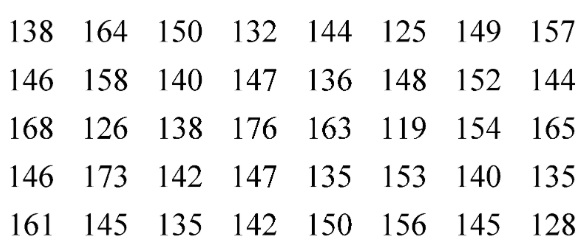
\includegraphics[scale=0.4]{images/1}
	\end{center}

	\begin{enumerate}
		\item Ordene los datos de menor a mayor y establezca el rango ($\varrho$) de los datos.
		\item Construya una tabla de distribución de frecuencias y asigne probabilidades (discretas) a cada intervalo asociado (Ayuda: Una elección conveniente para el tamaño del intervalo de clase es de 5lb.)
		\item Establezca las marcas de clase para cada uno de los intervalos de clase de la tabla de distribución de frecuencias anterior.
		\item En la misma tabla construya los intervalos con límites reales para las clases originales, conservando el tamaño y las marcas de clase de las mismas.
		\item Construya un histograma y un polígono de frecuencias asociada a la tabla de distribución de frecuencias.
	\end{enumerate}
	\item EXTRA: Repita el ejercicio anterior sólo que ahora con $c=8$. ¿Notó algún cambio en los resultados?
\end{enumerate}


%---------------------------
%\bibliographystyle{apa}
%\bibliography{referencias.bib}

\end{document}